\documentclass[11pt]{article}
\usepackage[margin=0.5in]{geometry}
\usepackage[utf8]{inputenc}
\usepackage{textcomp}

\usepackage{pgfplots}
\pgfplotsset{width=10cm,compat=1.9}

\usepackage{listings}
\usepackage{color}

\definecolor{dkgreen}{rgb}{0,0.6,0}
\definecolor{gray}{rgb}{0.5,0.5,0.5}
\definecolor{mauve}{rgb}{0.58,0,0.82}

\lstset{frame=tb,
  language=Java,
  aboveskip=3mm,
  belowskip=3mm,
  showstringspaces=false,
  columns=flexible,
  basicstyle={\small\ttfamily},
  numbers=none,
  numberstyle=\tiny\color{gray},
  keywordstyle=\color{blue},
  commentstyle=\color{dkgreen},
  stringstyle=\color{mauve},
  breaklines=true,
  breakatwhitespace=true,
  tabsize=3
}


%Gummi|065|=)
\title{\textbf{CO322 Data Structures and Algorithms\\Lab04 : Simple sorting algorithms}}
\vspace{3.5cm}
\author{E/14/158\\
		Gihan Chanaka Jayatilaka}
\date{20-04-2018}
\begin{document}

\maketitle
\clearpage

\tableofcontents
\clearpage

\section{Overview}

This report analyzes the following sorting algorithms.
\begin{itemize}
\item Bubble sort
\item Selection sort
\item Insertion sort
\end{itemize}

These algorithms were implemented on java and tested on integer \textbf{(int)} arrays of different sizes. The arrays were populated with random integers generated by java Random class with bounds of [0, twice the array size).\\

"Which algorithm is better?" depends on several factors such as,
\begin{itemize}
\item Accuracy of the algorithm
\item Code complexity of the algorithm
\item Efficiency of the algorithm
\end{itemize}

These factors can be evaluated both theoretically and experimentally.


\section{Algorithm implementation}
\subsection{Bubble sort}

\begin{lstlisting}
    static void bubble_sort(int [] data) {
        for(int iter=0;iter<data.length;iter++){
            boolean sorted=true;
            for(int x=0;x<data.length-1-iter;x++){
                if(data[x]>data[x+1]){
                    sorted=false;
                    swap(data,x,x+1);
                }
            }
            if(sorted)break;
        }
    }
\end{lstlisting}

\subsection{Selection sort}
\begin{lstlisting}
    static void selection_sort(int [] data) {
        for(int i=0;i<data.length-1;i++){
            int minIndex=i;
            for(int j=i+1;j<data.length;j++){
                if(data[minIndex]>data[j]){
                    minIndex=j;
                }
            }
            swap(data,i,minIndex);
        }
    }
\end{lstlisting}


\subsection{Insertion sort}
\begin{lstlisting}
    static void insertion_sort(int [] data) {
        for(int i=1;i<data.length;i++){
            for(int j=i-1;true;j--){
                if(j==-1|| data[i]>data[j]){
                    //circular swap operation
                    int temp=data[i];
                    for(int ii=i;ii>j+1;ii--)data[ii]=data[ii-1];
                    data[j+1]=temp;
                    break;
                }
            }
        }
    }
\end{lstlisting}



\section{Analysis factors}
\subsection{Accuracy of the algorithm}
The accuracy of all the algorithms considered in this exercise is 100\%. Therefor it is not a suitable comparison metric to choose the "better algorithm" in this case.

\subsection{Code complexity of the algorithms}
All three algorithms were implemented using \textbf{nested loops, comparison and swap} operations. The insertion sort has \textbf{circular swap} which is relatively complicated than the other algorithms.\\The code is fairly simple for all three algorithms. 


\subsection{Efficiency of algorithms}
Efficiency of an algorithm is the inverse of the resource consumption for the algorithm to run. The resources consumed are
\begin{itemize}
\item Computation time -- Time complexity
\item Memory -- Space complexity
\end{itemize}

Both these complexities could be analyzed theoretically or experimentally. In this report, the theoretical analysis is done for worst case scenarios \textbf{(Big Oh)}. The experimental analysis is done for \emph{average case} by generating the unsorted arrays by a uniform random distribution of integers.


\section{Theoretical analysis}

\subsection{No of operations}
\begin{tabular}{|c |c| c |c| c|}

\hline
Algorithm		&\multicolumn{2}{c}{Best case}		&\multicolumn{2}{c}{Worst case}\\
&No. of comparisions&No. of swaps&No. of comparisions&No. of swaps\\
\hline				
Bubble sort	&N-1	&0	&$\frac{N(N-1)}{2}$		&$\frac{N(N-1)}{2}$\\
\hline
Selection sort	&N-1	&0	&$\frac{N(N-1)}{2}$		&$\frac{N(N-1)}{2}$\\
\hline
Insertion sort	&$\frac{N(N-1)}{2}$	&0	&$\frac{N(N-1)}{2}$		&$\frac{N(N-1)}{2}$\\
\hline
\end{tabular}


\subsection{Big "O"}
\textbf{Note:}\\The space complexities are calculated by the additional space needed for the sort function. Since the unsorted array is passed by value in to the function, the space required for the array is neglected.\\

\begin{tabular}{|c|c|c|}
\hline
Algorithm & Time complexity & Space complexity\\
\hline
Bubble sort		&	$ O(N^2) $	&	$O(1)$		\\
Selection sort	&	$O(N^2)$	&	$O(1)$		\\
Insertion sort	&	$O(N^2)$	&	$O(1)$		\\
\hline
\end{tabular}


\section{Experimental}

\subsection{Procedure}

All three algorithms were evaluated against integer arrays of sizes \textbf{100, 1000, 5000, 10,000, 50,000 and 100,000}.
These arrays were filled by random numbers (from a uniform random distribution).
\\The 3 cases were chosen to be
\begin{itemize}
\item \textbf{Average case : }The randomly filled array.
\item \textbf{Best case : }The sorted array.
\item \textbf{Worst case : }The reversed array.
\end{itemize}


The time taken for an algorithm to sort (or identify the array as a sorted array in the best case scenarios) were measured by the System.currentTimeMillis() function in java.

\subsection{Results}
\subsubsection{Tabulated results for different order of N}


\begin{tabular}{|c||c|c|c||c|c|c||c|c|c|}
\hline
N&\multicolumn{3}{c}{Bubble sort}&\multicolumn{3}{c}{Selection sort}&\multicolumn{3}{c}{Insertion sort}\\
\hline
&Average & Best & Worst&Average & Best & Worst&Average & Best & Worst\\
&/(ms) &/(ms) &/(ms) &/(ms) &/(ms) &/(ms) &/(ms) &/(ms) &/(ms) \\
\hline

100&0&0&1&0&0&0&0&0&0\\
500&4&0&2&3&1&1&1&0&2\\
1000&1&0&1&0&1&3&3&0&3\\
5000&27&0&27&9&8&17&5&0&9\\
10000&130&0&103&34&33&82&21&0&34\\
50000&5130&0&2582&829&830&2192&430&0&856\\
100000&19837&1&10290&3328&3310&8783&1749&0&3608\\
\hline


\end{tabular}


\subsubsection{Results for different N in same order}

\begin{tabular}{|c||c|c|c||c|c|c||c|c|c|}
\hline
N&\multicolumn{3}{c}{Bubble sort}&\multicolumn{3}{c}{Selection sort}&\multicolumn{3}{c}{Insertion sort}\\
\hline
&Average & Best & Worst&Average & Best & Worst&Average & Best & Worst\\
&/(ms) &/(ms) &/(ms) &/(ms) &/(ms) &/(ms) &/(ms) &/(ms) &/(ms) \\
\hline

10000& 208 &0&170&59&55&84&38&0&44\\
20000& 756 &0&410&136&131&360&69&0&139\\
30000& 1831 &0&924&299&297&806&152&0&305\\
40000& 3224 &0&1638&531&527&1461&269&0&543\\
50000& 5069 &0&2559&826&817&2275&423&0&848\\
60000& 7385 &0&3693&1187&1177&3252&610&1&1225\\
70000& 10031 &0&5045&1617&1603&4427&831&0&1675\\
80000& 13116 &0&6548&2113&2097&5856&1094&1&2235\\
90000& 16657 &0&8287&2673&2659&7374&1400&1&2885\\
100000& 20648 &0&10262&3327&3293&9201&1733&0&3608\\

\hline


\end{tabular}


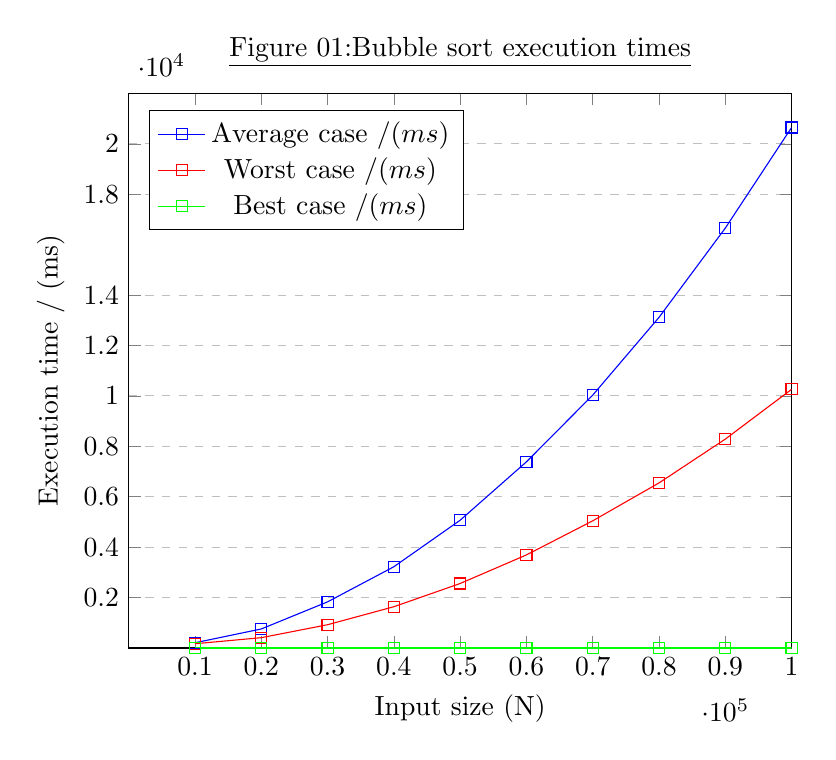
\begin{tikzpicture}
\begin{axis}[
    title={\underline{Figure 01:Bubble sort execution times}},
    xlabel={Input size (N)},
    ylabel={Execution time / (ms)},
    xmin=0, xmax=100000,
    ymin=0, ymax=22000,
    xtick={10000,20000,30000,40000,50000,60000,70000,80000,90000,100000},
    ytick={2000,4000,6000,8000,10000,12000,14000,66000,18000,20000},
    legend pos=north west,
    ymajorgrids=true,
    grid style=dashed,
]
 
\addplot[
    color=blue,
    mark=square,
    ]
    coordinates {
    (10000,208)(20000,756)(30000,1831)(40000,3224)(50000,5069)(60000,7385)(70000,10031)(80000,13116)(90000,16657)(100000,20648)
    };
    \addlegendentry{Average case /($ms$)}

\addplot[
    color=red,
    mark=square,
    ]
    coordinates {
    (10000,170)(20000,410)(30000,924)(40000,1638)(50000,2559)(60000,3693)(70000,5045)(80000,6548)(90000,8287)(100000,10262)
    };
    \addlegendentry{Worst case /($ms$)}  
    
\addplot[
    color=green,
    mark=square,
    ]
    coordinates {
    (10000,0)(20000,0)(30000,0)(40000,0)(50000,0)(60000,0)(70000,0)(80000,0)(90000,0)(100000,0)
    };
    \addlegendentry{Best case /($ms$)}    
     
\end{axis}
\end{tikzpicture}




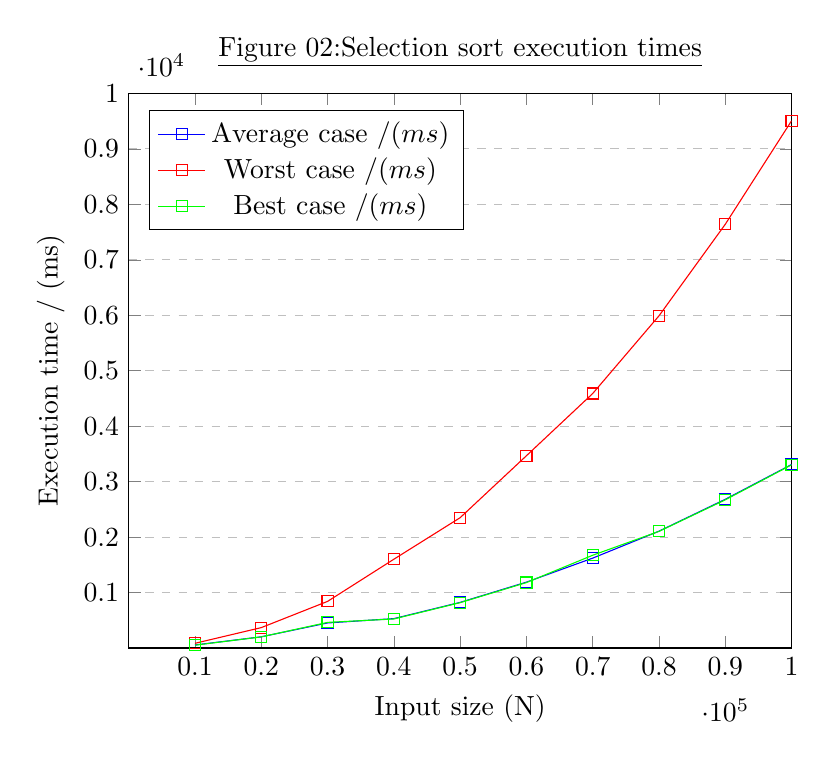
\begin{tikzpicture}
\begin{axis}[
    title={\underline{Figure 02:Selection sort execution times}},
    xlabel={Input size (N)},
    ylabel={Execution time / (ms)},
    xmin=0, xmax=100000,
    ymin=0, ymax=10000,
    xtick={10000,20000,30000,40000,50000,60000,70000,80000,90000,100000},
    ytick={1000,2000,3000,4000,5000,6000,7000,8000,9000,10000},
    legend pos=north west,
    ymajorgrids=true,
    grid style=dashed,
]
 
\addplot[
    color=blue,
    mark=square,
    ]
    coordinates {
(10000,55)(20000,202)(30000,452)(40000,530)(50000,823)(60000,1188)(70000,1621)(80000,2107)(90000,2682)(100000,3309)
    };
    \addlegendentry{Average case /($ms$)}

\addplot[
    color=red,
    mark=square,
    ]
    coordinates {
    (10000,85)(20000,368)(30000,841)(40000,1601)(50000,2350)(60000,3467)(70000,4589)(80000,5990)(90000,7641)(100000,9507)

    };
    \addlegendentry{Worst case /($ms$)}  
    
\addplot[
    color=green,
    mark=square,
    ]
    coordinates {
    (10000,51)(20000,201)(30000,462)(40000,524)(50000,818)(60000,1180)(70000,1673)(80000,2103)(90000,2672)(100000,3303)
    };
    \addlegendentry{Best case /($ms$)}    
     
\end{axis}
\end{tikzpicture}







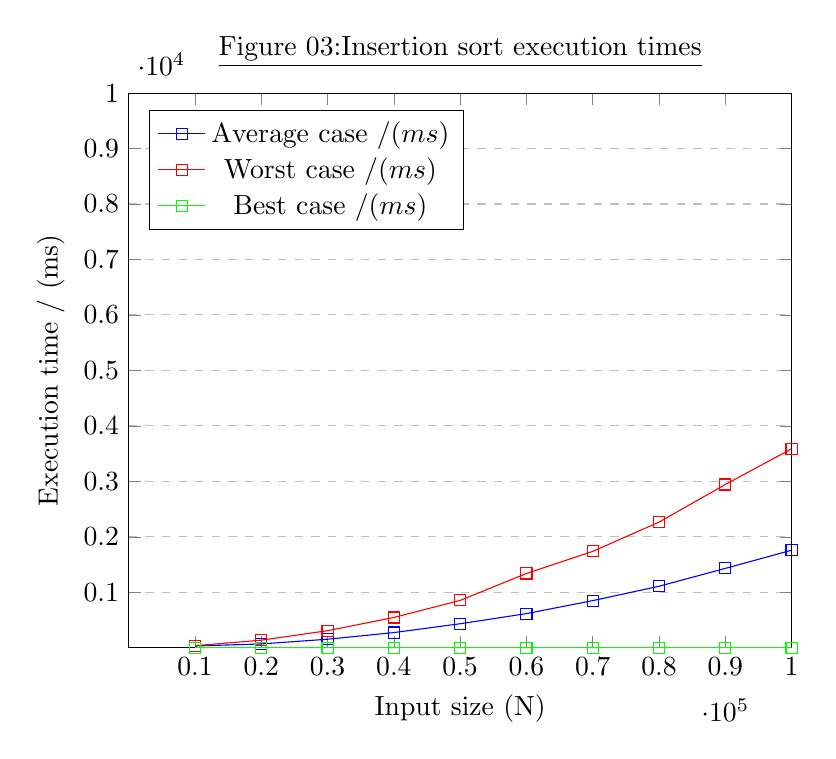
\begin{tikzpicture}
\begin{axis}[
    title={\underline{Figure 03:Insertion sort execution times}},
    xlabel={Input size (N)},
    ylabel={Execution time / (ms)},
    xmin=0, xmax=100000,
    ymin=0, ymax=10000,
    xtick={10000,20000,30000,40000,50000,60000,70000,80000,90000,100000},
    ytick={1000,2000,3000,4000,5000,6000,7000,8000,9000,10000},
    legend pos=north west,
    ymajorgrids=true,
    grid style=dashed,
]
 
\addplot[
    color=blue,
    mark=square,
    ]
    coordinates {
(10000,31)(20000,68)(30000,153)(40000,273)(50000,432)(60000,615)(70000,849)(80000,1108)(90000,1430)(100000,1758)
    };
    \addlegendentry{Average case /($ms$)}

\addplot[
    color=red,
    mark=square,
    ]
    coordinates {
(10000,36)(20000,136)(30000,307)(40000,545)(50000,853)(60000,1339)(70000,1737)(80000,2264)(90000,2943)(100000,3586)

    };
    \addlegendentry{Worst case /($ms$)}  
    
\addplot[
    color=green,
    mark=square,
    ]
    coordinates {
    (10000,0)(20000,0)(30000,0)(40000,0)(50000,0)(60000,1)(70000,0)(80000,0)(90000,1)(100000,1)
    };
    \addlegendentry{Best case /($ms$)}    
     
\end{axis}
\end{tikzpicture}


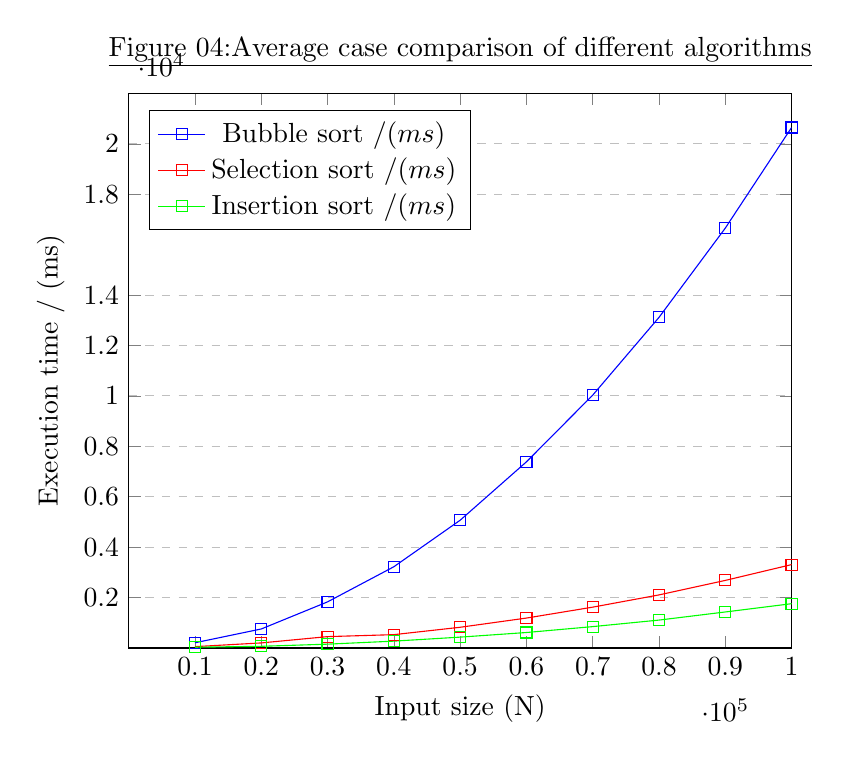
\begin{tikzpicture}
\begin{axis}[
    title={\underline{Figure 04:Average case comparison of different algorithms}},
    xlabel={Input size (N)},
    ylabel={Execution time / (ms)},
    xmin=0, xmax=100000,
    ymin=0, ymax=22000,
    xtick={10000,20000,30000,40000,50000,60000,70000,80000,90000,100000},
    ytick={2000,4000,6000,8000,10000,12000,14000,66000,18000,20000},
    legend pos=north west,
    ymajorgrids=true,
    grid style=dashed,
]
 
\addplot[
    color=blue,
    mark=square,
    ]
    coordinates {
    (10000,208)(20000,756)(30000,1831)(40000,3224)(50000,5069)(60000,7385)(70000,10031)(80000,13116)(90000,16657)(100000,20648)
    };
    \addlegendentry{Bubble sort /($ms$)}

\addplot[
    color=red,
    mark=square,
    ]
    coordinates {
(10000,55)(20000,202)(30000,452)(40000,530)(50000,823)(60000,1188)(70000,1621)(80000,2107)(90000,2682)(100000,3309)

    };
    \addlegendentry{Selection sort /($ms$)}  
    
\addplot[
    color=green,
    mark=square,
    ]
    coordinates {
(10000,31)(20000,68)(30000,153)(40000,273)(50000,432)(60000,615)(70000,849)(80000,1108)(90000,1430)(100000,1758)
    };
    \addlegendentry{Insertion sort /($ms$)}    
     
\end{axis}
\end{tikzpicture}


\subsection{Observations and conclusions}
\begin{itemize}
\item All sorting algorithms identify a sorted array and terminates very quickly except for the insertion sort.
\item The average time efficiency of the sorting algorithms increase in the order of\\ \textbf{Bubble $<$ Selection $<$ Insertion}.
\item The shape of $Time-N$ graphs match the theoretical prediction $O(N^2)$.
\item Surprisingly the \textit{worst case} is faster than the average case in Bubble sort.
\end{itemize}

\end{document}
